%%%%%%%%%%%%%%%%%%%%%%%%%%%%%%%%%%%%%%%%%
% Beamer Presentation
% LaTeX Template
% Version 1.0 (10/11/12)
%
% This template has been downloaded from:
% http://www.LaTeXTemplates.com
%
% License:
% CC BY-NC-SA 3.0 (http://creativecommons.org/licenses/by-nc-sa/3.0/)
%
%%%%%%%%%%%%%%%%%%%%%%%%%%%%%%%%%%%%%%%%%

%----------------------------------------------------------------------------------------
%	PACKAGES AND THEMES
%----------------------------------------------------------------------------------------

\documentclass[aspectratio=169]{beamer}
%\usepackage[ngerman]{babel}
\usepackage{amsmath}
\usepackage{bm}
\usepackage{amssymb}
\usefonttheme[onlymath]{serif}
\mode<presentation> {

% The Beamer class comes with a number of default slide themes
% which change the colors and layouts of slides. Below this is a list
% of all the themes, uncomment each in turn to see what they look like.

\usetheme{default}
%\usetheme{AnnArbor}
%\usetheme{Antibes}
%\usetheme{Bergen}
%\usetheme{Berkeley}
%\usetheme{Berlin}
%\usetheme{Boadilla}
%\usetheme{CambridgeUS}
%\usetheme{Copenhagen}
%\usetheme{Darmstadt}
%\usetheme{Dresden}
%\usetheme{Frankfurt}
%\usetheme{Goettingen}
%\usetheme{Hannover}
%\usetheme{Ilmenau}
%\usetheme{JuanLesPins}
%\usetheme{Luebeck}
\usetheme{Madrid}
%\usetheme{Malmoe}
%\usetheme{Marburg}
%\usetheme{Montpellier}
%\usetheme{PaloAlto}
%\usetheme{Pittsburgh}
%\usetheme{Rochester}
%\usetheme{Singapore}
%\usetheme{Szeged}
%\usetheme{Warsaw}

% As well as themes, the Beamer class has a number of color themes
% for any slide theme. Uncomment each of these in turn to see how it
% changes the colors of your current slide theme.

%\usecolortheme{albatross}
%\usecolortheme{beaver}
%\usecolortheme{beetle}
%\usecolortheme{crane}
%\usecolortheme{dolphin}
%\usecolortheme{dove}
%\usecolortheme{fly}
%\usecolortheme{lily}
%\usecolortheme{orchid}
%\usecolortheme{rose}
%\usecolortheme{seagull}
%\usecolortheme{seahorse}
%\usecolortheme{whale}
%\usecolortheme{wolverine}

%\setbeamertemplate{footline} % To remove the footer line in all slides uncomment this line
%\setbeamertemplate{footline}[page number] % To replace the footer line in all slides with a simple slide count uncomment this line

%\setbeamertemplate{navigation symbols}{} % To remove the navigation symbols from the bottom of all slides uncomment this line
}

\usepackage{graphicx} % Allows including images
\usepackage{booktabs} % Allows the use of \toprule, \midrule and \bottomrule in tables

%----------------------------------------------------------------------------------------
%	TITLE PAGE
%----------------------------------------------------------------------------------------

\title[Smart Services Development]{Implementation of a Home Automation Service} % The short title appears at the bottom of every slide, the full title is only on the title page

\author{Benedikt Görgei, Lukas D'Angelo, Patrick Eder} % Your name
\institute[] % Your institution as it will appear on the bottom of every slide, may be shorthand to save space
{
Technische Universität Graz \\ % Your institution for the title page
\medskip
\texttt{benedikt.goergei@student.tugraz.at, lukas.dangelo@student.tugraz.at, patrick.eder@student.tugraz.at} % Your email address
}
\date{\today} % Date, can be changed to a custom date

\begin{document}

\begin{frame}
\titlepage % Print the title page as the first slide
\end{frame}

\begin{frame}
\frametitle{Overview} % Table of contents slide, comment this block out to remove it
\tableofcontents % Throughout your presentation, if you choose to use \section{} and \subsection{} commands, these will automatically be printed on this slide as an overview of your presentation
\end{frame}

%----------------------------------------------------------------------------------------
%	PRESENTATION SLIDES
%----------------------------------------------------------------------------------------

%------------------------------------------------
\section{Introduction} % Sections can be created in order to organize your presentation into discrete blocks, all sections and subsections are automatically printed in the table of contents as an overview of the talk
%------------------------------------------------
\subsection{Aim and Motivation}
\begin{frame}
\frametitle{Aim and Motivation}
\begin{itemize}
\item Pre-existing network-enabled hardware I/O modules
\item General purpose inputs and outputs 
\item Sensor BUS
\item Building a smart service to control the hardware modules
\end{itemize}
\end{frame}

%------------------------------------------------
\section{Concept}
\subsection{Components}
%------------------------------------------------
\begin{frame}
\frametitle{Components}
\begin{figure}
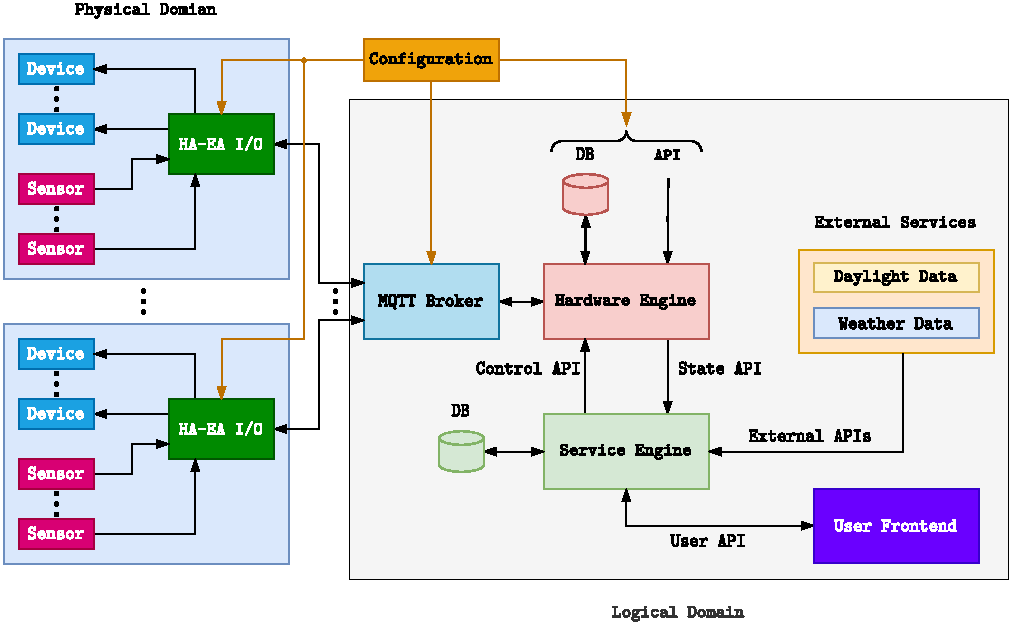
\includegraphics[width=0.65\linewidth]{./figures/specification.pdf}
\end{figure}
\end{frame}

%------------------------------------------------
\subsection{Services}
%------------------------------------------------
\begin{frame}
\frametitle{Components and Services}
\begin{itemize}
\item Physical domain
\begin{itemize}
\item Devices to control
\item Hardware I/O modules
\end{itemize}
\item Logical domain
\begin{itemize}
\item MQTT Broker
\item Hardware Engine
\item Service Engine
\item External Services
\item User Frontend
\end{itemize}
\end{itemize}
\end{frame}


%------------------------------------------------
\section{Implementation}
\subsection{Software Implementation}
%------------------------------------------------
\begin{frame}
\frametitle{Software Implementation}
\begin{itemize}
\item Communication Protocols
\begin{itemize}
\item MQTT for communicating with hardware
\item HTTP - REST
\end{itemize}
\item Programming Language and Frameworks
\begin{itemize}
\item Python 3
\item Flask 
\end{itemize}
\item Deployment - Docker:
\begin{itemize}
\item MQTT Broker
\item Hardware Engine
\item Service Engine and User Frontend
\end{itemize}

\end{itemize}
\end{frame}



%------------------------------------------------
\section{User Story and Demo}
\subsection{User Story}
%------------------------------------------------
\begin{frame}
\frametitle{User Story}
\begin{itemize}
\item We want to control the temperature of a room
\item An electrical valve is used to control the warm water flow of the radiators
\item A temperature sensor is used for temperature feedback
\item The sensor and the valve are connected to the I/O module
\end{itemize}
\end{frame}

\begin{frame}
\frametitle{User Story}
The user sets the following in the user interface:
\begin{itemize}
\item A target temperature (e.g. 21°C)
\item A time interval when heating should be done (e.g 08:00 - 20:00)
\item The weather conditions (e.g. not sunny, outdoor temperature  $<$ 5°C)
\end{itemize}
\end{frame}

%------------------------------------------------
\subsection{Demo}
%------------------------------------------------
\begin{frame}
\frametitle{Demo}

\begin{itemize}
 \item Service Engine API
 \item Graphical user interface
 \item Demo: Switching the light
\end{itemize}
\end{frame}

\begin{frame}
\Huge{\centerline{Thank you!}}
\Huge{\centerline{$\exists$ Questions?}}
\end{frame}

\end{document}